\documentclass{beamer}
\usetheme{Singapore}

% --------------------------------------------------------------------
% Packages pour la couleur
\usepackage{color}

% --------------------------------------------------------------------
% Packages pour les accents français.
\usepackage[latin1]{inputenc}	% L'option "latin1" désigne l'encodage ISO-8859-1, typique sous Linux.
\usepackage[T1]{fontenc}	% Pour les accents
\usepackage[frenchb]{babel}

% --------------------------------------------------------------------
% Voici certains packages souvent utilisés.
\usepackage{graphicx}		% Importation du package permettant d'inclure d'images dans le document.
\usepackage{amsmath, amsfonts}	% Pour écrire selon les standards de l'AMS.
\usepackage{epstopdf}		% Package permettant l'inclusion d'images eps, pour la compilation en pdf.
\usepackage{epsfig}
\usepackage{hyperref}
%\usepackage{subfig}
\usepackage{multirow}

% --------------------------------------------------------------------
% Le package "palatino" charge la police Palatino en mode texte et le package "euler" charge la police Euler en mode mathématique. Pour retrouver les polices par défaut, effacez les deux lignes de commandes qui suivent.
\usepackage{palatino}
\usepackage{euler}

% --------------------------------------------------------------------
% --------------------------------------------------------------------
% Commande rapide
\newcommand{\C}{\mathbb{C}}
\newcommand{\F}{\mathbb{F}}
\newcommand{\R}{\mathbb{R}}
\newcommand{\Q}{\mathbb{Q}}
\newcommand{\N}{\mathbb{N}}
\newcommand{\Z}{\mathbb{Z}}
\renewcommand{\H}{\mathcal{H}}
\renewcommand{\O}{\mathcal{O}}

\newcommand{\abcdmat}{\begin{pmatrix}
a & b \\ 
c & d
\end{pmatrix}}
\newcommand{\ida}{\mathfrak{a}}
\newcommand{\idb}{\mathfrak{b}}
\newcommand{\idc}{\mathfrak{c}}
\newcommand{\p}{\mathfrak{p}}
\newcommand{\tha}{\theta_\mathfrak{a}}
\newcommand{\thb}{\theta_\mathfrak{b}}
\newcommand{\tpsi}{\theta_\psi}
\newcommand{\ClK}{\text{Cl}_K}

\newtheorem{thm}{Theorem}
\newtheorem{defn}[thm]{Definition}
\newtheorem{prop}[thm]{Proposition}
\newtheorem{coro}[thm]{Corollary}
\newtheorem{lem}[thm]{Lemma}
\newtheorem{conj}[thm]{Conjecture}
\newtheorem{rem}[thm]{Remark}
\newtheorem{ex}[thm]{Example}
\newtheorem{qu}{Question}

%Groupe modulo
\newcommand*{\modulo}[2]
{\raisebox{.6ex}{ \newline \ensuremath{#1}}\!/\!\raisebox{-.6ex}{\ensuremath{#2}}}

% --------------------------------------------------------------------
% --------------------------------------------------------------------
% --------------------------------------------------------------------

\title{Petersson Inner Product of Binary Theta Series}
\subtitle{A computational approach}
\author{Nicolas \textsc{Simard}}
\institute{McGill University}
\date{September 17th, 2016}


\begin{document}

\frame{
	\titlepage
}

%\AtBeginSection[]
%{
%  \begin{frame}
%    \frametitle{Table of Contents}
%    \tableofcontents[currentsection]
%  \end{frame}
%}

\section{Introduction and Background}
\subsection{Introduction}
\frame{
	\frametitle{Motivation: Stark's remark}
	In the last paragraph of his well-known article \emph{"L-functions at $s=1$. II. Artin L-functions with Rational Characters"}, Stark makes the following remark:
	\begin{quotation}
		An application of Theorem $1$ gives
		\[L'(0,\chi,H/\Q) = \log\epsilon,\]
		where $\epsilon$ is the real root of
		\[x^3-x-1=0\]
		Actually, it is easier to note that $L(1,\chi,H/\Q)$ is the residue at $s=1$ of the zeta function of the real quadratic subfield of $K$. In any case,
		\[\langle f,f\rangle = 3\log\epsilon.\]
	\end{quotation}
}

\subsection{Modular forms}
\frame{
	\frametitle{Mobius transformations}
Let $\H$ be the Poincar\'e upper-half plane. Recall that $\text{GL}_2(\R)_+$ acts on $\H$ via Mobius transformations:
\[\abcdmat z=\frac{az+b}{cz+d}.\]
\begin{defn}
	Let $N\geq1$ and define the Hecke subgroup of level $N$ as
	\[\Gamma_0(N)=\left\lbrace\abcdmat \in\text{SL}_2(\Z)| c\equiv 0\pmod N\right\rbrace.\]
\end{defn}
	
}

\frame{
	\frametitle{Level $N$ modular forms with characters}

\begin{defn}
	Let $N\geq1$ and $k\geq0$ be integers and let $\chi$ be a Dirichlet character mod $N$. A modular form of weight $k$, level $N$ and character $\chi$ is a holomorphic function
	\[f:\H\longrightarrow\C\]
	such that
	\[f\left(\frac{az+b}{cz+d}\right)=\chi(d)(cz+d)^kf(z)\]
	for all $z\in\H$ and all $\gamma\in\Gamma_0(N)$, which satisfies certain growth conditions at the cusps.	The $\C$-vector-space of such modular forms is denoted
	\[M_k(\Gamma_0(N),\chi).\]
\end{defn}
}	
	
\frame{
	\frametitle{$q$-expansion of modular forms}
	Every modular form $f$ has a Taylor (or Fourier) expansion at infinity, called its $q$-expansion:
	\[f(z)=\sum_{n=0}^\infty a_nq^n,\]
	where $q=exp(2\pi iz)$. If
	\[a_0(f)=0,\]
	(at all cusps) $f$ is called a \emph{cusp form}. The space of cusp forms is denoted
	\[S_k(\Gamma_0(N),\chi).\]
}

\frame{
	\frametitle{Example: weight $k$ Eisenstein series}
	Let $k\geq4$ be an even integer. Then the series
	\[\sum_{m,n}\frac{1}{(mz+n)^k}\]
	converges absolutely and defines a modular form in $M_k(\text{SL}_2(\Z))$. After renormalization, the $q$-expansion of this Eisenstein series is
	\[-\frac{B_k}{2k}+\sum_{n=1}^\infty\sigma_{k-1}(n)q^n:=G_k(z),\]
	where
	\[\sigma_{k-1}(n)=\sum_{d|n}d^{k-1}.\]
}

\frame{
	\frametitle{Important non-example: weight $2$ Eisenstein series}
	In level $1$, there are no modular forms of weight $2$. However, one can still define the weight $2$ Eisenstein series as
	\[G_2(z)=\frac{1}{8\pi\Im(z)}-\frac{1}{24}+\sum_{n=1}^\infty\sigma(n)q^n.\]
	It is an example of an \emph{almost holomorphic} modular form of level $1$ and weight $2$.
}

\subsection{Spaces of modular forms}
\frame{
	\frametitle{Finite dimensionality of spaces of modular forms}
	\begin{theorem}
		The space $M_k(\Gamma_0(N),\chi)$ is finite dimensional as a $\C$-vector-space.
	\end{theorem}
	\begin{ex}
	In level $N=1$, we have
	\begin{itemize}
		\item $M_0(\text{SL}_2(\Z))=\C$.
		\item $M_2(\text{SL}_2(\Z))=0$.
		\item $M_k(\text{SL}_2(\Z))=\C G_k$ for $4\leq k\leq 10$.
		\item $M_{12}(\text{SL}_2(\Z))=\C G_{12}\oplus\C\Delta$, where $\Delta\in S_{12}(\text{SL}_2(\Z))$.
		\item $\bigoplus_{k=0}^\infty M_k(\text{SL}_2(\Z))=\C[G_4,G_6]$.
	\end{itemize}
	\end{ex}
}

\frame{
	\frametitle{Petersson inner product}
	Let $f,g\in S_k(\Gamma_0(N),\chi)$ be two cusp forms. The Petersson inner product of $f$ and $g$ is defined as
	\[\langle f,g\rangle =\int\int_{\Gamma_0(N)\setminus\H}f(x+iy)\overline{g(x+iy)}y^k\text{d}\mu,\]
	where
	\[\text{d}\mu=\frac{\text{d}x\text{d}y}{y^2}\]
	is the $\text{SL}_2(\R)$-invariant measure on $\H$.
	Note that the integral does not converge if neither $f$ nor $g$ is a cusp form.
}

\section{Theta Series}
\subsection{The simplest example}
\frame{
	\frametitle{A half-integral weight theta series}
	Consider the function
	\[\theta(z) = \sum_{x\in\Z}q^{x^2}=1+2q+2q^4+O(q^5).\]
	Then
	\[\theta(\gamma z)=\epsilon(cz+d)^{1/2}\theta(z),\]
	for all $\gamma\in\Gamma_0(4)$ and some $\epsilon_{c,d}\in\lbrace\pm1,\pm i\rbrace$.
}

\subsection{Theta series attached to imaginary quadratic fields}
\frame{
	\frametitle{Theta series attached to ideals}
	Let $K$ be an imaginary quadratic field of discriminant $D<-4$ and let $\O_K$ be its ring of integers. Fix an integer $\ell\geq0$.
	
	To each integral ideal $\ida$ of $K$, one can attach the following theta series:
	\[\tha^{(2\ell)}(z)=\tha(z)=\sum_{x\in\ida}x^{2\ell}q^{N(x)/N(\ida)}.\]
	
}

\frame{
	\frametitle{Basic properties of these theta series}
	\begin{enumerate}
		\item<1-> We have
		\[\tha=\sum_{x\in\ida}x^{2\ell}q^{N(x)/N(\ida)}\in M_{2\ell+1}(\Gamma_0(|D|),\chi_D),\]
		where $\chi_D$ is the Kronecker symbol. If $\ell\neq0$, then
		\[\tha\in S_{2\ell+1}(\Gamma_0(|D|),\chi_D).\]
		\item<2-> If $\lambda\in K^\times$, then
		\[\theta_{\lambda\ida}=\lambda^{2\ell}\tha.\]
		So there are essentially $h_K$ theta series attached to $K$.
		\item<3-> In general, the $\tha$ are \emph{not} newforms.
	\end{enumerate}
}

\frame{
	\frametitle{Theta series attached to Hecke characters of $K$}
	Let $I_K$ denote the group of fractional ideals of $K$. A Hecke character $\psi$ of $K$ of infinity type $2\ell$ (and conductor $1$) is a homomorphism
	\[\psi:I_K\longrightarrow \C^\times\]
	such that
	\[\psi((\alpha))=\alpha^{2\ell},\hspace{1cm}\forall\alpha\in K^\times.\]
	One can define
	\[\tpsi=\sum_{\ida\subseteq\O_K}\psi(\ida)q^{N(\ida)}.\]
}

\frame{
	\frametitle{Basic properties of these theta series}
	\begin{enumerate}		
		\item<1-> We have
		\[\tpsi\in M_{2\ell+1}(\Gamma_0(|D|),\chi_D),\]
		where $\chi_D$ is the Kronecker symbol. If $\psi^2\neq 1$, then
		\[\tpsi\in S_{2\ell+1}(\Gamma_0(|D|),\chi_D).\]
		\item<2-> The $\tpsi$ are newforms, so
		\[\langle\tpsi,\theta_{\psi'}\rangle=0\]
		whenever $\psi\neq\psi'$.
		\item<3-> We have the identities
		\[\tpsi=\frac{1}{w_K}\sum_{[\ida]\in\ClK}\psi^{-1}(\ida)\tha\hspace{0.5cm}\text{and}\hspace{0.5cm}\tha=\frac{w_K}{h_K}\sum_{\psi}\psi(\ida)\tpsi.\]
	\end{enumerate}
}

\frame{
	\frametitle{Stark's example}
	To obtain Stark's example, take
	\[K=\Q(\sqrt{-23})\]
	and let $\psi$ be a non-trivial Hecke character of infinity type $0$, i.e. a non-trivial character of the class group. Then
	\[\text{Stark's }f =\text{our }\tpsi\in M_1(\Gamma_0(23),\chi_{-23}).\]
}

\subsection{Some questions}
\frame{
	\frametitle{Some questions}
	Keeping Stark's example in mind, we have the following questions:
	\begin{itemize}
		\item Can we find explicit formulas for the Petersson inner product of those theta series (whenever it makes sense)?
		\item Can we efficiently compute it?
		\item Can we use those formulas/computations to study the arithmetic properties of those quantities?
	\end{itemize}
	\only<2->{
	The main question is
	\begin{qu}
		Can we $p$-adically interpolate those formulas for $\ell>0$ and take the limit as $\ell\rightarrow 0$ $p$-adically to obtain the weight one case?
	\end{qu}
	}
}

\section{Explicit formulas}
\subsection{The case $\ell=0$}
\frame{
	\frametitle{The case $\ell=0$}
	\begin{theorem}
		Let $\tpsi$ be a Hecke character of infinity type $0$ and suppose that $\psi^2\neq 1$. Then
		\begin{align*}
		\langle\tpsi,\tpsi\rangle 	&= -h_K\sum_{[\ida]\in\ClK}\psi^2(\ida)\log(\Im(\tau_\ida)^{1/2}|\eta(\tau_\ida)|^2)\\
									&= h_K\log\prod_{[\ida]\in\ClK}(\Im(\tau_\ida)^{1/2}|\eta(\tau_\ida)|^2)^{-\psi(\ida)^2}.
		\end{align*}
	\end{theorem}
	Here,
	\[\tau_\ida=\omega_2/\omega_1\in\H\]
	if $\ida=\Z\omega_1\oplus\Z\omega_2\subset\C$ is positively oriented ideal in $K$ and
		\[\eta(z)=exp(2\pi i/24)\prod_{n=1}^\infty(1-q^n).\]
	
}

\subsection{The case $\ell>0$}
\frame{
	\frametitle{Petersson norm of the $\tpsi$ (with $\ell>0$)}
	\begin{theorem}
		Let $\psi$ be a Hecke character of $K$ of infinity type $2\ell$, where $\ell>0$. Then
		\[\langle\tpsi,\tpsi\rangle = h_K(|D|/4)^\ell\sum_{[\ida]\in\ClK}\psi^2(\ida)\partial^{2\ell-1}G_2(\ida).\]
	\end{theorem}
	Here,
	\[\partial f=\frac{1}{2\pi i}\frac{\partial f}{\partial z}-\frac{k}{4\pi\Im(z)}f\]
	is the Shimura-Mass differential operator, which preserves the graded algebra of almost holomorphic modular forms.
}

\frame{
	\frametitle{Petersson inner product of the theta series $\tha$}
	\begin{theorem}
		Let $\ida$ and $\idb$ be ideals of $K$ and suppose $\ell>0$. Then
		\[\langle\tha,\thb\rangle=C_K^{(2\ell)}N(\idb)^{2\ell}\sum_{\ida\idb^{-1}\idc^2=\lambda_\idc\O_K}\lambda_\idc^{2\ell}\partial^{2\ell-1}G_2(\idc),\]
		where
		\[C_K^{(2\ell)}=4(|D|/4)^\ell.\]
	\end{theorem}
}

\frame{
	\frametitle{A few direct consequences of the formula}
	\begin{coro}
		For $\ell>0$,
		\[\langle\tha,\thb\rangle=0\]
		whenever $\ida$ and $\idb$ are not in the same genus (i.e. the classes of $\ida$ and $\idb$ are distinct in the genus group $\ClK/\ClK^2$).
	\end{coro}
	\begin{coro}
		For $\ell>0$,
		\[\langle\theta_{\ida\idc},\theta_{\idb\idc}\rangle=N(\idb\idc)^{2\ell}\langle\tha,\thb\rangle.\]
	\end{coro}
}

\frame{
	\frametitle{An arithmetic consequence}
	Let
	\[\Omega_K=\frac{1}{\sqrt{4\pi|D|}}\left(\prod_{j=1}^{|D|-1}\Gamma\left(\frac{j}{|D|}\right)^{\chi_D(j)}\right)^{w_K/4h_k}\]
	be the Chowla-Selberg period attached to $K$.
	\begin{coro}
		For $\ell>0$, the complex numbers
		\[\frac{\langle\tpsi,\tpsi\rangle}{\Omega_K^{4\ell}}\hspace{0.5cm}\text{and}\hspace{0.5cm}\frac{\langle\tha,\thb\rangle}{\Omega_K^{4\ell}}\]
		are algebraic.
	\end{coro}
}

\subsection{The case $\ell=0$ revisited}
\frame{
	\frametitle{Formally obtaining the case $\ell=0$ from the case $\ell>0$}
	Strictly speaking, the formula
	\[\langle\tpsi,\tpsi\rangle = h_K(|D|/4)^\ell\sum_{[\ida]\in\ClK}\psi^2(\ida)\partial^{2\ell-1}G_2(\ida).\]	
	does not make sense for $\ell=0$, since the expression
	\[\partial^{-1}G_2\]
	is not well-defined. However, we observe that
	\[\partial_0 \log(\Im(z)^{1/2}|\eta(z)|^2)=-G_2(z),\]
	so
	\["\partial^{-1}G_2(z)=-\log(\Im(z)^{1/2}|\eta(z)|^2)"\]
	and we \emph{formally} obtain the case $\ell=0$ from the case $\ell>0$.
}

\subsection{A remark on using the formula}
\frame{
	\frametitle{Computing $\partial^nG_2$}
	To compute
	\[\partial^nG_2\]
	we have the following formulas:
	\[\partial G_2=\frac{5}{6}G_4-2G_2^2 \hspace{0.5cm}\partial G_4 = \frac{7}{10}G_6-8G_2G_4\hspace{0.5cm}\partial G_6 = \frac{400}{7}G_4^2-12G_2G_6.\]
	For example,
	\[\partial^3G_2=-48G_2^4 + 120G_4G_2^2 - 14G_6G_2 + 25G_4^2.\]
}

\section{Numerical computations}
\subsection{Examples of computations}

\frame{
	\frametitle{Class number $1$ case}
	In this case,
	\[\theta_{\O_K}=\theta_{\psi_0}\]
	and we only need to compute
	\[\langle\theta_{\O_K},\theta_{\O_K}\rangle/\Omega_K^{4\ell}\in\overline{\Q}.\]
}

\frame{
	\frametitle{Class number $1$ case}
	Computation of $\langle\theta_{\O_K},\theta_{\O_K}\rangle/\Omega_K^{4\ell}$:
	\renewcommand{\arraystretch}{1.25}
	\begin{tabular}{cc|*{2}{l|}}
	\cline{3-4}
	& & \multicolumn{2}{ c| }{$\ell$} \\ \cline{3-4}
	& & 1 & 2 \\ \cline{1-4}
	\multicolumn{1}{ |c| }{\multirow{7}{*}{$D$}} & \multicolumn{1}{ |c| }{-7}
	&$2^{2}3$&$-2^{2}$\\
	\cline{2-4}
	\multicolumn{1}{ |c| }{}&\multicolumn{1}{ |c| }{-8}
	&$-2$&$-2^{2}5$\\
	\cline{2-4}
	\multicolumn{1}{ |c| }{}&\multicolumn{1}{ |c| }{-11}
	&$-2^{2}$&$-2^{3}5$\\
	\cline{2-4}
	\multicolumn{1}{ |c| }{}&\multicolumn{1}{ |c| }{-19}
	&$-2^{2}3^{-1}13$&$-2^{3}71$\\
	\cline{2-4}
	\multicolumn{1}{ |c| }{}&\multicolumn{1}{ |c| }{-43}
	&$-2^{3}3^{-1}107$&$-2^{4}5647$\\
	\cline{2-4}
	\multicolumn{1}{ |c| }{}&\multicolumn{1}{ |c| }{-67}
	&$-2^{2}3^{-1}7^{2}31$&$-2^{3}5\cdot86629$\\
	\cline{2-4}
	\multicolumn{1}{ |c| }{}&\multicolumn{1}{ |c| }{-163}
	&$-2^{3}3^{-1}150473$&$-2^{4}11\cdot461681471$\\
	\cline{1-4}
	\end{tabular}
}

%\frame{
%	\frametitle{Class number $2$}
%	In this case, $K$ has two genera. If $\ida$ is a representative of the non-trivial class in $\ClK$, we have
%	\[\langle\theta_\ida,\theta_{\O_K}\rangle = \langle\theta_{\O_K},\theta_\ida\rangle=0\]
%	and
%	\[\langle\theta_\ida,\theta_\ida\rangle=N(\ida)^{2\ell}\langle\theta_{\O_K},\theta_{\O_K}\rangle,\]
%	so it suffices to compute the quantity
%	\[\langle\theta_{\O_K},\theta_{\O_K}\rangle/\Omega_K^{4\ell}\in\overline{\Q}.\]
%}
%
%\frame{
%	\frametitle{Class number $2$}
%	As in the class number $1$ case, the quantity
%	\[\langle\theta_{\O_K},\theta_{\O_K}\rangle/\Omega_K^{4\ell}\]
%	is an integer, except for $\ell=1$ and $D=-91,-403$ and $-427$.
%}

\frame{
	\frametitle{$K=\Q(\sqrt{-23})$ (class number $3$, one genus): $\ell=0$}
	For $\psi$ a non-trivial Hecke character of infinity type $0$, the explicit formula in case $\ell=0$ gives
	\[\langle f,f\rangle=\langle\tpsi,\tpsi\rangle=3\log \epsilon,\]
	where
	\[\epsilon=\prod_{[\ida]\in\ClK}(\Im(\tau_\ida)^{1/2}|\eta(\tau_\ida)|^2)^{-\psi(\ida)^2}\]
	is the real root of
	\[x^3-x-1\]
	and generates the Hilbert class field of $K$.
}

\frame{
	\frametitle{$K=\Q(\sqrt{-23})$ (class number $3$, one genus): $\ell>0$}
	In $K$, the prime $2$ splits as
	\[2\O_K=\p_2\bar{\p}_2\]
	and
	\[\ClK=\lbrace 1,[\p_2],[\bar{\p}_2]\rbrace.\]
	Moreover, we have $\langle\theta_{\bar{\p}_2},\theta_{\O_K}\rangle=\overline{\langle\theta_{\p_2},\theta_{\O_K}\rangle}$, so we only care about
	\[\langle\theta_{\p_2},\theta_{\O_K}\rangle\hspace{0.5cm}\text{and}\hspace{0.5cm}\langle\theta_{\O_K},\theta_{\O_K}\rangle.\]
}

\frame{
	\frametitle{$K=\Q(\sqrt{-23})$ (class number $3$, one genus): $\ell>0$}
	Consider the algebraic number
	\[a(\ell)=\langle\theta_{\O_K},\theta_{\O_K}\rangle/\Omega_K^{4\ell}.\]
	For $\ell=1,2$ and $4$, we find that $a(\ell)^3$ is a root of a monic cubic polynomial and generates the Hilbert class field over $K$. 
	\begin{ex}
	$a(1)$ is a root of the polynomial
	\[x^9 - 2816x^6 - 905216x^3 - 89915392.\]
	\end{ex}
}

\frame{
	\frametitle{$K=\Q(\sqrt{-23})$ (class number $3$, one genus): $\ell>0$}
	Consider the algebraic number
	\[a(\ell)=\langle\theta_{\O_K},\theta_{\O_K}\rangle/\Omega_K^{4\ell}.\]
	For $\ell=3,6$ and $9$, we find that $a(\ell)$ is a root of a cubic polynomial and generates the Hilbert class field over $K$.
	\begin{ex}
	$a(3)$ is a root of
	\[x^3 - 6740x^2 - 169034720x - 1027491892288.\]
	\end{ex}
}

\frame{
	\frametitle{$K=\Q(\sqrt{-23})$ (class number $3$, one genus): $\ell>0$}
	A few computations of the Gramm matrix for this basis.
	\begin{tabular}{|c|c|}
	\hline
	$\ell$ & $\det(\langle\theta_{\ida_i}^{(2\ell)},\theta_{\ida_j}^{(2\ell)}\rangle)_{\ida_i,\ida_j\in\ClK}/(\Omega_K^{4\ell})^3$ \\
	\hline
	$1$ & $-2^{10}23$ \\
	\hline
	$2$ & $-2^{14}19\cdot23\cdot619$ \\ 
	\hline
	$3$ & $-2^{18}5^{2}11\cdot23\cdot337\cdot27299$ \\ 
	\hline
	$4$ & $-2^{22}7^{2}23\cdot163\cdot2113\cdot117741979$ \\ 
	\hline
	$5$ & $-2^{26}5^{3}23\cdot229\cdot23761\cdot808991\cdot20338663$ \\ 
	\hline
	$6$ & $-2^{30}5^{2}11^{2}13\cdot19\cdot23\cdot67^{2}101\cdot868697\cdot505912247899$ \\ 
	\hline
	\end{tabular}
}

\frame{
	\frametitle{$K=\Q(\sqrt{-23})$ (class number $3$, one genus): $\ell>0$}
	Consider now the algebraic number
	\[N(\psi,\ell) = \langle\theta_{\psi},\theta_{\psi}\rangle/\Omega_K^{4\ell}\]
	For $\ell=1,2,4$ and $5$, the numbers $N(\psi_i,\ell)$, for $0\leq i\leq 2$, are distinct and their cube are the three real roots of a monic cubic polynomial. 
	\begin{ex}
		The numbers $N(\psi_i,1)^3$, for $0\leq i\leq 2$, are the three roots of the irreducible polynomial
	\[x^3 - 6966x^2 + 11569230x - 239483061.\]
	\end{ex}
}

\frame{
	\frametitle{$K=\Q(\sqrt{-23})$ (class number $3$, one genus): $\ell>0$}
	Consider now the algebraic number
	\[N(\psi,\ell) = \langle\theta_{\psi},\theta_{\psi}\rangle/\Omega_K^{4\ell}\]
	For $\ell=3,6$ and $9$, one of the characters, say $\psi_0$, the algebraic number $N(\psi_0,\ell)$ is an \emph{integer}. For the two others, we find that their cube are the roots of a monic quadratic polynomial.
	\begin{ex}
	We have
	\[N(\psi_0,3) = 5055 = 3\cdot5\cdot337\]
	and $N(\psi_1,3)^3$ and $N(\psi_2,3)^3$ are the roots of
	\[x^2 - 16287872873193x + 30021979248651078296845875.\]
	\end{ex}
}
\frame{
	\frametitle{$K=\Q(\sqrt{-23})$ (class number $3$, one genus): $\ell>0$}
	A few computations of the Gramm matrix for this basis.
	\begin{tabular}{|c|c|}
	\hline
	$\ell$ & $\det(\langle\theta_{\psi_i},\theta_{\psi_j}\rangle)_{1\leq i,j\leq 3}/(\Omega_K^{4\ell})^3$ \\
	\hline
	$1$ & $-3^{3}23$ \\
	\hline
	$2$ & $-3^{3}19\cdot23\cdot619$ \\ 
	\hline
	$3$ & $-3^{3}5^{2}11\cdot23\cdot337\cdot27299$ \\ 
	\hline
	$4$ & $-3^{3}7^{2}23\cdot163\cdot2113\cdot117741979$ \\ 
	\hline
	$5$ & $-3^{3}5^{3}23\cdot229\cdot23761\cdot808991\cdot20338663$ \\ 
	\hline
	$6$ & $-3^{3}5^{2}11^{2}13\cdot19\cdot23\cdot67^{2}101\cdot868697\cdot505912247899$ \\ 
	\hline
	\end{tabular}
}

\subsection{Is the algorithm efficient?}
\frame{
	\frametitle{Example of computation for $K=\Q(\sqrt{-23})$: $N(\psi_0,3)$}
	\begin{figure}
		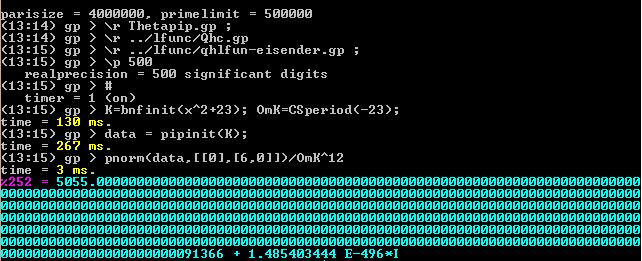
\includegraphics[scale=0.65]{example2.jpg}
	\end{figure}
}

\section{Idea of the proof}
\subsection{Idea of the proof}
\frame{
	\frametitle{Main steps in the proof (case $\ell>0$)}
	\begin{enumerate}
		\item<1-> Use Rankin-Selberg to prove that
		\[\langle\tpsi,\tpsi\rangle=\textcolor{gray}{\frac{4h_k}{w_k}\sqrt{|D|}\frac{\Gamma(2\ell+1)}{(4\pi)^{2\ell+1}}}L(\psi^2,2\ell+1).\]
		\item<2-> Relate Hecke L-series to non-holomorphic Eisenstein series:
		\[L(\psi^2,2\ell+1)=\frac{1}{w_K}\sum_{[\ida]\in\ClK}\frac{\psi^2(\ida)}{N(\ida)^{4\ell-s}}G_{4\ell}(\ida,1-2\ell).\]
		\item<3-> Replace non-holomorphic Eisenstein series by derivatives of Eisenstein series:
		\[\partial^{2\ell-1}G_2(z)=\textcolor{gray}{(-4\pi)^{1-2\ell}\frac{\Gamma(s+2\ell+1)}{\Gamma(s+2)}}G_{4\ell}(z,1-2\ell).\]
		\item<4-> Find $\langle\tha,\thb\rangle$ using $\langle\tpsi,\tpsi\rangle$.
	\end{enumerate}
}

\section{Conclusion}
\subsection{Conclusion}
\frame{
	\frametitle{What we would like to know}
	\begin{enumerate}
		\item Can we explain what can be observed from the computations?
		\item Can we say something about the Petersson inner product of non-cuspidal weight one theta series?
		
	\end{enumerate}
	\only<2->{
	But again, the main question remains
	\begin{qu}
		Can we $p$-adically interpolate the formulas for $\ell>0$ and take the limit as $\ell\rightarrow 0$ $p$-adically to obtain the weight one case?
	\end{qu}
	}
}

\frame{
	\frametitle{Thank you!}
	
	Presentation available at: \url{https://github.com/NicolasSimard/Notes/tree/master/PANTS\%20XXVI}
	
	Code available at : \url{https://github.com/NicolasSimard/ENT}
	
	Notes available at:\url{https://github.com/NicolasSimard/Notes/tree/master/Theta\%20Norm}
}

\end{document}
